\lhead{\emph{Active Magnetic Compensation Prototype}}
\chapter{Active Magnetic Compensation Prototype}\label{ch:amcP}
% \printinunitsof{pt}\prntlen{\textwidth}

% In Chapter~\ref{ch:magnetics}, the requirements of the magnetic field for nEDM experiment have been discussed. It also includes the active magnetic compensation to stabilize the external magnetic field. This thesis is based on the development of Active Compensation system for the TUCAN nEDM experiment. For that purpose a 


A prototype active magnetic compensation system was built and tested at the University of Winnipeg. This chapter describes the components of the prototype and their performance. Measurements of time-dependence of the surrounding field in the laboratory are also presented. The system was designed to compensate fluctuations of that relevant scale. In Chapter~\ref{ch:operation}, I then discuss the multi-dimensional feedback algorithm which corrects fluctuations.


% The chapter describes the Active Magnetic Field Compensation (AMC) prototype that has been built at the University of Winnipeg. All the apparatus that made the AMC prototype will be discussed in detail.

\section{Overview of AMC Prototype}\label{sec:amcp_overview}
% This Section gives an overview of the AMC prototype that has been built at the University of Winnipeg in the development process of implementing the original one at TUCAN nEDM experiment.


\doublefig{Images/exp4}{width=0.95\textwidth,height =8cm}{Schematic diagram \label{fig:exp}}{Images/exp_photo}{width =0.95\textwidth,height =8cm}{Photograph\label{fig:exp_photo}}{{Active Magnetic Field Compensation (AMC) Prototype at University of Winnipeg. The schematic diagram is shown in (a) and a photograph in (b). Surrounding the outermost mu-metal passive shielding layer are six coils on six faces of a cubic $\mathrm{Al}$ frame. A seventh coil provides additional perturbations to the field. The magnetic environment is sensed by the 3-axis fluxgates placed at various positions near the shield and coil system. A fourth order low-pass Butterworth filter removes high-frequency noise. Fluxgate signals are recorded by an ADC and a computer uses a multi-dimensional feedback algorithm to control the currents in the coils via DAC's and current sinks.} \label{fig:active}}{Active Magnetic Field Compensation (AMC) Prototype at University of Winnipeg}


A schematic diagram of the prototype is displayed in Fig.~\ref{fig:active}\textcolor{blue}{(a)}. A picture of the coils and magnetic shield is shown in Fig.~\ref{fig:active}\textcolor{blue}{(b)}. The magnetic background fluctuation was known to be $\sim100$~nT (see Section~\ref{sec:field}) over the course of a day. The prototype has been designed to compensate that by introducing six current carrying single loop coils on the six faces of a cube frame. The frame surrounds the outermost mu-metal shield of a four-layer cylindrical passive shielding system. A seventh square coil was used to generate additional perturbations. The properties of the mu-metal shields are discussed further in Section~\ref{sec:shield} and the coil cube in Section~\ref{sec:cube}. 

Four 3-axis fluxgate sensors were placed at positions near the shield and coil system to measure the field for compensation. Another 3-axis fluxgate sensor was placed at the center of the passive shield for quantification of the prototype. Details of the fluxgate sensor system are discussed in Section~\ref{sec:sensor}.


%\FloatBarrier
% \clearpage
The fluxgates suffered from environmental noise dominated by 60~Hz electrical noise. Moreover, if the system has any potential of generating noise at $\sim8$~Hz in a $1~\mu$T field, it could induce changes in the $\mathrm{^{199}Hg}$ free precession. A $\mathrm{4^{th}}$-order low-pass Butterworth filter with corner frequency 10~Hz was built to reduce the noise. The filter details are prescribed in Section~\ref{sec:filter}. After filtering, the signals are transmitted to the computer via the analog to digital converter (ADC) of a LabJack T7 Pro~\cite{T7}. The required currents are calculated in a PC using a proportional-integral (PI) control algorithm. The computer uses digital to analog converters (DACs) to control six voltage controlled current sinks. The current sinks drive the six compensation coils.

% \fig{Images/exp2}{width = 0.8\textwidth}{Schematic diagram of prototype active compensation system at University of Winnipeg.\label{fig: active}}
I now discuss in more detail each component of the system.

\section{Mu-Metal Shields}\label{sec:shield}
The passive magnetic shielding is composed of thin multi-layer shields with materials having high magnetic permeability (mu-metal). 

% The outer layers are usually cylindrical \cite{mu_cyl_1,mu_cyl_2} but they can also take the same forms as the magnetic shielded room (msr)~\cite{mu_msr_1,mu_msr_2}. The inner layer is designed based on the coil to achieve required homogeneity \cite{mu_inner_1,mu_inner_2}. 

\fig{Images/passive2}{width =0.95\textwidth}{Prototype passive shielding at University of Winnipeg~\cite{mammei_presentation}.\label{fig: passive}}{Prototype passive shielding at University of Winnipeg}


In the prototype at UW, there are four layers of cylindrical shields enclosing a volume of interest as shown in Fig.~\ref{fig: passive}. Each shell is enclosed  with end caps as shown in Fig.~\ref{fig: passive}\textcolor{blue}{(a)}. Amumetal (Magnifer 7904) of thickness 0.0625 inch has been used for the layers,  which is an 80\% Nickel-Iron alloy. The shields were fabricated and annealed by Amuneal Manufacturing Corp.~\cite{mu-metal}.  There are two end-caps in each cylinder with a 7.5~cm diameter in the central hole. To minimize the leakage of the external fields into the progressively shielded inner volumes, a stove-pipe of length 5.5~cm is placed on each hole (see Fig.~\ref{fig: passive}\textcolor{blue}{(a)}).

\begin{table} [!htb]
    \centering
    \begin{tabular} { |c|c|c|c|c|c|} 
        \hline
        Parameters & Innermost Layer & $\mathrm{2^{nd}}$ Layer & $\mathrm{3^{rd}}$ Layer & Outermost Layer & Stove Pipe\\
        \hline\hline
        Radius (cm) & 18.5 & 23.5 & 30 & 38 & 3.7 \\ 
        \hline
        Length (cm) & 37 & 55 & 71 & 90 & 5.5 \\ 
         \hline
    \end{tabular}
    % \vspace{4mm}
    \caption[Dimensions of prototype passive shielding layers]{Dimensions of prototype passive shielding layers including stove pipes radius and length.}\label{table:mu-metal}
\end{table}

The radii and lengths of the four layers including the stove pipes are shown in Table~\ref{table:mu-metal}. A combined DC shielding factor $\sim\mathrm{10^6}$ is expected. A discussion about another prototype of similar design but smaller in size can be found in Ref. \cite{baby_shield}, where the shielding factor $=\mathrm{10^7}$ was measured using a very sensitive magnetometer.



% %\FloatBarrier
% The above discussion gives an idea about the dimensions and properties of the prototype passive shielding at the University of Winnipeg. Next the coil cube will be discussed in details.

\section{Coil Cube}\label{sec:cube}

\fig{Images/coil}{width =0.9\textwidth}{Schematic diagram indicating the coil   configuration and the position of the fluxgate sensors.\label{fig:coil}}{Schematic diagram indicating the coil configuration and the position of the fluxgate sensors.}

As discussed in Section~\ref{sec:amcp_overview}, the prototype has been designed to compensate $\sim 100$~nT magnetic background fluctuations by introducing six current carrying closed loop coils on six faces of a cube surrounding the outermost mu-metal shield. The coils are designated as $C_x^\pm$, $C_y^\pm$ and $C_z^\pm$ (Fig.~\ref{fig:coil}) and are sometimes referred to as compensation coils because they are responsible for compensating magnetic fluctuations. The side length of the cube is 1.15~m. In addition, there is a perturbation coil namely $P_z^+$, which is used to apply additional field for testing purposes. Figure~\ref{fig:coil} also displays the numbers 1-8 indicating possible positions of the fluxgate sensors, which will be discussed in the next section.


\begin{table} [!htb]
    \centering
    \begin{tabular} { |c|c|c| } 
        \hline
        Parameters & \makecell{Compensation Coils \\ ($C_x^\pm$, $C_y^\pm$ and $C_z^\pm$)} & \makecell{Perturbation Coil \\ ($P_z^+$)} \\
        \hline\hline
        Dimension (m$\times$m) & 1.15$\times$1.15 & 1.15$\times$1.15\\ 
        \hline
        No. of Turns & 1 & 77\\ 
        \hline
        Resistance ($\Omega$) & 0.15 & 11.55\\ 
        \hline
        Inductance (mH) & 0.32 & 24.62\\
        % \hline
        % Current ($A$) & 0 & 1\\
         \hline
    \end{tabular}
    % \vspace{4mm}
    \caption{Coil dimensions and electrical properties.}\label{table:coil}
\end{table}

% \FloatBarrier
The compensation coils have been chosen to be single turn to have small resistance ($\sim0.15~\Omega$) and small inductive reactance. The perturbation electro-magnet coil has the same dimensions but 77 turns. The perturbation coil was typically placed in the same face as $C_z^+$ and separated from it by 1.06~m. Coil properties are summarized in Table~\ref{table:coil}. 


% %\FloatBarrier
% The above discussion gives an idea about the coil configuration, dimensions and properties. Next, the apparatus used to measure magnetic field will be discussed.


\section{Fluxgate Sensors}\label{sec:sensor}
% The measured data from the fluxgate sensors are transferred to the computer via anlog to digital converter (ADC) of LabJack T7 Pro which will be discussed in the next section. But before coming to the ADC, the 3-axis of the fluxgates have to be separated and for that purpose we have build  2 breakout boxes. 

% A breakout box was built to separate each of $x$, $y$ and $z$ axis in respective direction and provide power. 
A fluxgate sensor is a piece of magnetic material, within a sensing winding used for measuring the magnitude and direction of DC or low-frequency AC magnetic fields. The magnetometer's sensitivity direction is the axis of the sensing winding. The magnetic material is periodically saturated by a source of excitation power. It is the transition of this material into magnetic saturation that creates the measurement signal.


\begin{table} [!htb]
    \centering
    \begin{tabular} { |c|c|c|c|c|c|} 
        \hline
        Parameters & Mag-03 & Mag690 \\
        \hline\hline
        Measure Range ($\mu$T) & $\pm$70 & $\pm$100 \\ 
        \hline
        \makecell{Noise Level \\($\mathrm{pT_{rms}\;/\sqrt{Hz}}$ at 1~Hz)} & $<6$ & $10~-<20$ \\ 
        \hline
        Bandwidth (kHz) & 3 & 1 \\ 
        \hline

    \end{tabular}
    % \vspace{4mm}
    \caption{Properties of the fluxgate sensors used for the prototype.}\label{table:sensor}
\end{table}

For the prototype, I have used four 3-axis fluxgate sensors (2 Bartington Mag-03 and 2 Bartington Mag690) placed at different positions within the compensation coils to measure field for compensation. Beside those, one 3-axis fluxgate sensor (Bartington Mag690) has been placed at the center of the prototype for quantification of it's performance. The numbering 1-8 in Fig.~\ref{fig:coil} indicates possible positions of the fluxgates. I also tried more positions which will be discussed in Chapter~\ref{ch:quantification}. A breakout box was built to separate each of $x$, $y$ and $z$ axis of the fluxgates in respective direction and provide power. The breakout box separates both powers and four 3-axis fluxgate sensors resulting in $3\times4=12$ analog outputs. Figure~\ref{fig:coil} also defines the direction $x$, $y$ and $z$ for the fluxgates.  The properties of the fluxgate sensors that I have used for the prototype are shown in Table~\ref{table:sensor} and collected from the manufacturer~\cite{flux}. 



%\FloatBarrier

\fig{Images/noise}{width =0.8\textwidth}{Average Spectral Density for Mag690. \label{fig:noise}}{Average Spectral Density for Mag690.}

According to the manufacturer, the typical noise levels are from $\mathrm{<6~pT_{rms}\;/\sqrt{Hz}}$ and $\mathrm{10}-\mathrm{<20}$~$\mathrm{pT_{rms}\;/\sqrt{Hz}}$ at $\mathrm{1~Hz}$ for Mag-03 and Mag690 respectively. I measured the noise levels of the fluxgate and found they matched the manufacturer's specification. For my test, data was taken by placing each fluxgate inside the shield and field data recorded. The data was processed in Mathematica~\cite{Mathematica} to estimate the power spectral density using a Discrete Fourier Transform (DFT)~\cite{dft}. Figure~\ref{fig:noise} shows that the noise level is $\sim\mathrm{16~pT_{rms}\;/\sqrt{Hz}}$ at $\mathrm{1~Hz}$ for the Mag690. This also confirms that the ADC (Section~\ref{sec:DAQ}) doesn't present any substantial noise beyond the fundamental noise of the fluxgate.




% The above discussion gives an idea about the definition of the fluxgate sensor and the properties of the fluxgate sensors that we hav used. Next in the list according to Fig.~\ref{fig:active}\textcolor{blue}{(a)}, we should discuss the filter. But the necessity of the filter came later and so the data acquisition process will be discussed  where the analog to digital converter (ADC) and digital to analog converter (DAC) are the main components.


\section{Data Acquisition (DAQ) Module}\label{sec:DAQ}

The signals from the fluxgates are all analog. An analog to digital converter (ADC) transfers information to the computer and a digital to analog converter (DAC) transfers information out of the computer. For that purpose, I used a LabJack T7 Pro Data Acquisition (DAQ) device~\cite{T7}.

\subsubsection{ADC of LabJack T7 Pro}

The signals that are measured by fluxgate sensors are separated into $x$, $y$ and $z$ axis via breakout box and then with/without filter (discussed later) are transmitted to the computer via ADC of LabJack T7 Pro. The ADC records the analog voltage in terms of ADC counts. An ADC count is the smallest change in the voltage for a single change in ADC value. The resolution of ADC defines the number of discrete voltages which can be represented for a input range. 

% For example, an ADC with 16 bit resolution can record $\mathrm{2^16=65536}$ discrete voltages and for an input range of 10 V, the smallest change in the voltages will be $\mathrm{10}$ V$\mathrm{/2^16=0.153}$ mV. But it is just theoretical prediction considering no channel noise. But in reality, in addition to noise of the ADC itself, there are noises from the power source and the fluxgates which contribute to the channel resolution and that resolution is called effective resolution which is lower than ideal resolution.


In addition to the standard 16-bit ADC with range $\pm10~\mathrm{V}$, the LabJack T7-Pro is equipped with a 24-bit sigma-delta ADC. The effective resolution can be varied from 16 to 19.1~bits when analog conversions occur on the 16-bit ADC and for 24-bit it is from 19.6 to 21.8 bits with gain 1~\cite{T7}. For testing, I used a short jumper to connect a test channel with ground and 512 successive reading and mean of those readings were stored. The root mean square calibrated voltage differences from the mean was calculated as $\mathrm{\Delta V_{rms}}$. This was converted to bits using
\begin{equation}
    \mathrm{Effective\;Resolution=log_2\left(\frac{\Delta V_{fsr}}{\Delta V_{rms}}\right)}
\end{equation}
where, $\mathrm{\Delta V_{fsr}=20~V}$ is the ADC full-scale range for $\mathrm{gain=1}$ used for this study.
% The root mean square of the differences between the mean of the readings with each reading was calculated and termed as $\mathrm{noise_{rms}}$. Depend on the 16-bit or 24-bit ADC with their input range, $\mathrm{noise_{rms}}$ had been converted into ADC counts which transformed into bits by multiplying with $\mathrm{log_2}$ and termed as $\mathrm{noise_{bits}}$. The effective resolution was finally calculated by subtracting $\mathrm{noise_{bits}}$ from either  16 bits or 24 bits resolution depend on the type of ADC. For example, for a 16-bit ADC with $\pm$10~V range, the noise in terms of bits and thus effective resolution:
% \begin{equation}\label{eq:adc_mean}
%     \mathrm{noise_{bits}=log_2 \times \left(\frac{noise_{rms}\times 2^{16}}{20}\right)}
% \end{equation}

% \begin{equation}
%     \mathrm{Effective\;Resolution=16 - noise_{bits}}
% \end{equation}. 

\fig{Images/res_T7adc}{width =0.75\textwidth}{Effective resolution for different resolution index for gain 1 and $\pm 10\:V$ range. A higher resolution index will result in lower noise and higher effective resolution but increases sample times. \label{fig:res}}{Effective resolution for different resolution index for gain 1 and $\pm 10\:V$ range.}



% After finding out the ADC counts of $\mathrm{noise_{rms}}$, the corresponding bits has been found by multiplying with $\mathrm{log_2}$.  Finally, the effective resolution was found by subtracting that amount of bit form either the 16 bit or 24 bit ADC depends on which one is used. In short the formula \cite{T7} for 16-bit ADC will be
% \begin{equation}
%     \mathrm{Effective\;Resolution=16\;bits - [log_2 \times mean_{rms} (in\;ADC \;counts)]\;bits}
% \end{equation}
% And for 24 bit sigma-delta ADC will be
% \begin{equation}
%     \mathrm{Effective\;Resolution=24\;bits - [log_2 \times mean_{rms} (in\;ADC \;counts)]\;bits}
% \end{equation}


Figure~\ref{fig:res} compares the manufacturer~\cite{T7} result (dashed red) with my measured result (solid green) for different resolution indices. Higher resolution index means lower noise but also increases averaging and decreases bandwidth. Table~\ref{table:t7freq2} shows this. Normally, gain 1(first column of Table~\ref{table:t7freq2}) was used.



% It is seen from the figure that the results are quite similar. Note that for resolution index 1-8, T7 Pro uses 16-bit ADC and for 9-12 resolution index it uses 24-bit sigma-delta ADC. 
\begin{table} [!htb]
    \centering
    \begin{tabular} { |c|c|c|c|c| } 
        \hline
        \thead{Res. Index} & \makecell{Bandwidth (Hz) \\ (Gain/Range: \\ 1/$\pm$ 10V)} & \makecell{Bandwidth (Hz) \\ (Gain/Range: \\ 10/$\pm$ 1V)} & \makecell{Bandwidth (Hz) \\ (Gain/Range: \\ 100/$\pm$ 0.1V)} & \makecell{Bandwidth (Hz) \\ (Gain/Range: \\ 1000/$\pm$ 0.01V)}\\
        \hline\hline
        1 & 25000.0 & 4347.8 & 970.9 & 198.8\\ 
        \hline
        2 & 25000.0 & 4347.8 & 492.6 & 100.0\\ 
        \hline
        3 & 16666.7 & 1818.2 & 198.0 & 99.0\\ 
        \hline
        4 & 11111.1 & 1724.1 & 196.9 & 99.0\\ 
        \hline
        5 & 6250.0 & 869.6 & 194.2 & 98.0\\ 
         \hline
        6 & 3448.3 & 438.6 & 97.3 & 97.1\\ 
        \hline
        7 & 1785.7 & 392.2 & 94.8 & 94.3\\ 
        \hline
        8 & 917.4 & 324.7 & 90.3 & 90.1\\ 
         \hline
        9 & 285.7 & 285.7 & 285.7 & 285.7\\ 
        \hline
        10 & 74.6 & 74.6 & 74.6 & 74.6\\ 
        \hline
        11 & 15.1 & 15.1 & 15.1 & 15.1\\ 
         \hline
        12 & 6.3 & 6.3 & 6.3 & 6.3\\ 
         \hline
         
    \end{tabular}
    % \vspace{4mm}
    \caption[T7 Pro manufacturer's sample frequency for different resolution index]{T7 Pro sample frequency for different resolution index, gain and voltage range~\cite{T7}.}\label{table:t7freq2}
\end{table}

% After having idea about the LabJack T7 Pro ADCs, now sampling frequency will be discussed. Note from the above that, the time required for the ADC hardware to make a single analog to digital conversion on any channel is ADC sampling time which doesn't include command/response and overhead time associated with the host computer/application~\cite{T7}. And the inverse of this ADC sampling time is called the sampling frequency. In normal mode, the ADC can sample as low as 6.3 Hz to 25 kHz per sample as shown in Table \ref{table:t7freq2}. Sampling at 6.3 Hz, the ADC itself is capable of avoiding all sorts of noises due its long average time. But the more channels means less sample frequency which makes the system more slower.



%\FloatBarrier
\begin{table} [!htb]
    \centering
    \begin{tabular} { |c|c|c|c|c| } 
        \hline
        \thead{Res. Index} & \makecell{Loop bandwidth (Hz)\\for 1 channel\\ (Gain/Range: 1/$\pm$ 10V)}& \makecell{Loop bandwidth (Hz)\\for 14 channels\\ (Gain/Range: 1/$\pm$ 10V)}& \makecell{Possible Averages \\for 14 channels\\ to meet design goal}\\
        \hline\hline
        1 & 3846.2 & 344.7 & 50\\ 
        \hline
        2 & 3846.2 & 328.0 & 48\\ 
        \hline
        3 & 3448.3 & 303.2 & 45\\ 
        \hline
        4 & 2777.8 & 263.8 & 39\\ 
        \hline
        5 & 2272.7 & 209.4 & 31\\ 
         \hline
        6 & 1694.9 & 149.4 & 23\\ 
        \hline
        7 & 1204.8 & 95.3 & 15\\ 
        \hline
        8 & 694.4 & 55.4 & 9\\ 
         \hline
        9 & 237.5 & 19.5 & 3\\ 
        \hline
        10 & 71.6 & 5.3 & -\\ 
        \hline
        11 & 15.0 & 1.1 & -\\ 
         \hline
        12 & 6.3 & 0.4 & - \\ 
         \hline
         
    \end{tabular}
    % \vspace{4mm}
    \caption[T7 Pro measured loop frequency for different resolution index]{T7 Pro loop frequency for different resolution index with gain 1 achieved in my setup at U.Winnipeg. Possible loop bandwidth for 14 channels and software averaging to meet design goal is also shown.}\label{table:t7freq}
\end{table}
% For the prototype, by effective sampling frequency we meant that the number of signals of the fluxgate sensors that are going to the feedback algorithm via analog to digital converter (ADC) per second per measurement. But we are recording the time for a complete iteration which we call it as loop sampling frequency which includes the ADC effective sampling frequency plus rest of the loop frequency. 

Table~\ref{table:t7freq2} reports sampling rate for each analog input. If more than one input is used , the overall sample rate suffers accordingly since the same ADC is used. In addition, there are computer delays. Including these delays results in a lower frequency which I call the loop sampling frequency (Table~\ref{table:t7freq}). For resolution index 1, it is found to be 3846.2~Hz, which is smaller than the effective sampling frequency 25000~Hz reported in Table~\ref{table:t7freq2} because of polling time which is typically 1~ms per channel read~\cite{T7}. The polling time includes LJM library overhead, Linux overhead, USB communication time, and device processing time. Table~\ref{table:t7freq} also shows the possible loop bandwidth for 14 fluxgate axes that I have used for active magnetic compensation. Possible software averaging is also shown in Table~\ref{table:t7freq} to meet the 6~Hz system design goal. Resolution index $1-9$ are acceptable to meet the design goal. Software averaging should give roughly the same noise performance which is discussed later (Chapter~\ref{ch:quantification}).
%\FloatBarrier
% The above discussion shows that the effective resolution that the LabJack corporation has given in their website are pretty similar to our result (see Fig.~\ref{fig:res}) and if we want to sample faster we need a lower resolution index but that will increase noise. To get rid of that noise and to meet design goal we can use software averaging (see Table~\ref{table:t7freq}), and filters which will be discussed in the latter part of this chapter.

\subsubsection{LabJack T7 Pro with LJTick-DAC}
Once the fluxgate signals have been processed in the PI control algorithm within the computer, currents must be sent to the compensation coils. An expansion module from LabJack called the LJTick-DAC provides two 14-bit analog outputs per module with a range of $\pm10$~V. The LJTick-DAC plugs into any digital I/O block of T7 Pro. To control the seven coils (including the perturbation coil), I used 4 LJTick-DACs connected to LabJack T7 Pro via the CB15 terminal. 

% There are 3 LJTickDACs each with two channels thus total six for six compensation coils. They are shown in Fig. \ref{fig:tick}.

% \fig{Images/dac}{width =  \textwidth, height =6 cm}{LJTickDAC \label{fig:tick}}

% The DACs have 14 bits of resolution over $\pm$10 V range. For the prototype, there should be a current source that can convert DACs voltage to current so that 100 nT cna be generated. So, a current sink has been designed in the half of the range of DACs voltage. The currents required can be found by -

% \begin{equation}\label{eq:iSink}
%     I_{out}^{sink}=V\times nT^{-1}/R
% \end{equation}
% So, for 100 nT the required current according to Eq. \ref{eq:iSink} is -
% \begin{equation}\label{eq:iSink_100}
%     I_{out}^{sink}=10\times 100^{-1}/50=200\:mA
% \end{equation}

% This ends our discussion of DAQ for now. Next, we will test the resolution of the DAC as claimed by the LabJack by doing experiment on it after describing the current sink circuit.


\section{Current Sink}\label{sec:sink}


The LJTick-DACs provide 14-bit analog outputs with a range of $\pm10$~V. The analog outputs are voltage signals which must be converted to currents for the coils. An 8-channel current sink device was built which will be discussed in this section. 

% To generate the designed $\sim 200\:nT$ magnetic field by the coils (see section \ref{sec:cube}), it was found that $\sim 200\:mA$ current must be sent to them. So, a current sink  device as shown in Fig. \ref{fig:currenSink} with 8 channels has been built.

% The 8 channels are actually 8 different voltage controlled current source circuits whose output currents are controlled by their input voltages. The circuit actively monitors and regulates the voltage drop across its sense resistor ($\mathrm{R_{sense}}$) until that is equal to the incoming voltage (in this case the output voltage of the LJTickDACs). Now, the the coil is kept in series with this resistor and thus, whatever current flows through the sense resistor must also flow through the coil. The device is termed as current sink device as current flows into the coils. The current sinks were designed to control 0-200 mA current from a 10V signal range. Because, 


It was found that the field generated by one of the coils at the center of the cube was $\sim200$~nT, when there was $\sim200$~mA current flowing through the coil. Since the environmental magnetic fluctuations are $\sim100$~nT, a $200$~mA current sink was considered sufficient. The required gain of the current sink is then such that $200$~mA current shall be generated over a $10$~V range. In the current sink design (Fig.~\ref{fig:currenSink}), it means that the sense resistor must be $\mathrm{R_{sense}=\frac{10~V}{0.2~A}=50~\Omega}$. Of the eight available channels, six were connected to the six compensation coils and our first prototype current sink was connected to the perturbation coil. Other two remaining channels are not instrumented. The 8-channel device is powered by $24$~V at a limit of $\sim 1.3$~A current. 

\fig{Images/currentSink2}{width =0.9\textwidth}{Current Sink Device. Circuit diagram of one of the voltage controlled current sink device shows in (a) and the pictorial topview of all the assembled current sink circuits shows in (b). The description is given in the text. \label{fig:currenSink}}{Current Sink Device}


% In the circuit diagram of one of the voltage controlled current sink is shown in Fig.~\ref{fig:currenSink}\textcolor{blue}{(a)}. It is seen that the output voltage from LJTick-DAC$\_$1a (channel a of first LJTick-DAC) is coming to the non-inverting input of an operational-amplifier (op-amp) and inverting input of that op-amp is connected to the sense resistor. The output of the op-amp is connected pin 1 (also known as gate) of a power metal-oxide-semiconductor field-effect transistor (MOSFET) designed for low voltage, high
% speed switching applications. So, voltage from LJTick-DAC$\_$1a ($\mathrm{V_{in}}$) is coming to gate of MOSFET and also current is generated as $\mathrm{I_{out}=V_{in}/R_{sense}}=V_{in}/50$ where, $\mathrm{Vin}$ ranges from 0 to 10 V. Now, when voltage between pin 1 (gate G) and pin 3 (source S) of MOSFET i.e.  $\mathrm{V_{GS}>0}$, then $\mathrm{I_{out}}$ flows from pin 3 (source S) to pin 2 (drain D) and eventually flows towards the coil $C_x^-$. It is also seen that a Schottky diode has been connected in parallel with the output where coil $C_x^-$ is connected for reverse current protection. It should be noted that outputs can not be left open. All the current sink circuits are assembled in a box and a picture from top is shown in Fig.~\ref{fig:currenSink}\textcolor{blue}{(b)}.


In the circuit diagram (Fig.~\ref{fig:currenSink}\textcolor{blue}{(a)}), the output voltage from LJTick-DAC$\_$1a (channel a of first LJTick-DAC) is connected to the input of the current sink. The output of the op-amp is connected to pin 1 (the gate) of a power metal-oxide-semiconductor field-effect transistor (MOSFET) designed for low voltage, high speed switching applications. A Schottky diode is connected in parallel with the output where the coil $C_x^-$ is connected for reverse current protection. All the current sink circuits are assembled in a box and a picture is shown in Fig.~\ref{fig:currenSink}\textcolor{blue}{(b)}.

% For calibrating current sink device, currents in the range of $0-200$ mA was requested and on the basis of that DACs generate the required voltages. Then the DACs generated voltage (input voltage) and the current that has been requested have been measured by 34970A data acquisition device. The readings of the input voltage and measured current have been noted. A linear fit of the input voltage (y-axis) based on LabJack 24-bit sigma-delta ADC specifications and measured current (x-axis) was made. The slope and offset of that fit is the ultimate gain and offset of the current sink channels. The gain found was 50 as expected because $\mathrm{R_{sense}}$ is 50 $\Omega$.  

The current sinks were calibrated and agreement was formed with the gain of $50~\Omega$ set by $\mathrm{R_{sense}}$.  

% Although the LJTickDACs support a $\pm10$~V range, the current sink device has been built to be in 0-10 V range. The reason is that it is relatively easy to make a circuit that can source or sink current based on a unipolar voltage and unipolar current. However, to generate a circuit that can do both without any distortion near $0\:V$ is a bit harder but certainly doable. But losing half ranges was not an issue for the prototype design and thus without wasting time, the device was built. Now, at this point, if it is required to utilize the full resolution of the DACs,  it's probably easier to just modify the LJTick-DACs $\pm$10 V range to a smaller range prior to the generation of the bipolar output instead of making a new voltage controlled current supply. The first LJTick-DAC had been done modified in this way. 

Although the LJTickDACs support a $\pm10$~V range, the current sink device uses the $0-10$~V range for convenience, at the cost of losing one bit in resolution. If it is required to utilize the full resolution of the DACs,  it's probably easier to just modify the LJTick-DACs $\pm10$~V range to a smaller unipolar range which exists on the chip just prior to the generation of the bipolar. We succesfully modified one LJTick-DAC in this way, and modified $\mathrm{R_{sense}}$ accordingly in its current sink. 

% For testing the resolution of the DACs, 500 values in the range of  0-1 mA was requested with 0.001 mA increment each time and the currents have been measured by 34970A data acquisition device. The readings of measured current had been noted.Then, the differences between the successive measured currents (mA)  were calculated from which the average difference was determined. Finally, from that average difference the resolution of the DACs had been calculated as
% \begin{equation}
% \mathrm{Resolution\;of\;DAC= log_2\left(\frac{200}{Measured\;Current\;Average\;Difference}\right)\;bits}
% \end{equation}
% where, 200 came from the fact that for full range of LJTick-DAC, the current sink produced 0-200 mA current.

The current resolution was tested using an Agilent 34970A data acquisition device with an ammeter module in it. Results are shown in Fig.~\ref{fig:dac} and are in agreement with expectation.

\fig{Images/dacRes2}{width=0.95\textwidth}{Resolution of LJTick-DACs. Currents measured (vertical-axis) with 0.001~mA increment each time  for requested current (horizontal axis) from 0 to 1~mA to find the resolution of the DACs. Resolution of channel b of modified LJTick-DAC is shown in (a), and resolution of channel b of unmodified LJTick-DAC in (b).\label{fig:dac}}{Resolution of LJTick-DACs}

% The resolution of channel b of modified first LJTick$\_$DAC is shown in Fig.~\ref{fig:dac}\textcolor{blue}{(a)}. It is seen that we have found 14 bits resolution as expected from the modified one. Again, the resolution of channel b of unmodified second LJTick$\_$DAC is shown in Fig.~\ref{fig:dac}\textcolor{blue}{(b)}. It is seen that the resolution is 13 bits in this case.


% The above discussion is all about the current sink that we have built. Next we will talk about a filter which is also built by us.





\section{Filtering}\label{sec:filter}

The raw fluxgate signals have a large amount of $60$~Hz noise. In principle, the ADC can handle this by increasing the amount of averaging. This is done by increasing the resolution index (Table~\ref{table:t7freq}) but at the cost of a slower effective sampling rate (bandwidth). The noise was large enough that resolution index 12 needed to be used which was unacceptably slow, and insufficient to meet the 6~Hz design goal for the long correction rate. 

% We have built twelve $\mathrm{4^{th}}$-order low-pass Butterworth filter with an aim to reduce noise while increasing sample rate for our fluxgate sensors. A low-pass filter has a constant gain (ratio between output and input) from 0 Hz to a high cutoff frequency where gain is down by 3 dB and after that the gain decreases with increasing input frequency. The frequencies between 0 Hz and the high cutoff frequency is known as passband frequencies whereas after that the frequencies are in stopband region. We use Butterworth filter approximation as they have flat passband and flat stopband. The specification of our filter are shown in Table~\ref{table:butter}. We have chosen the voltage range to be $\pm$12 V which is the same for our fluxgate sensors. So, we can use the same power supply for both the filter and the fluxgates. The precession frequency of $\mathrm{^{199}Hg}$ co-magnetometer for nEDM experiment in a 1$\mu$T field is $\sim$8 Hz~\cite{bea}. We only concern about the noises around this frequency. Because, if the system has any potential of generating noise at the $\mathrm{^{199}Hg}$ precession frequency in a 1 uT field, it could induce changes in the $\mathrm{^{199}Hg}$ free precession. In addition of cancelling 60 Hz electrical noise, because of low $\mathrm{^{199}Hg}$ precession frequency, we select the cutoff frequency of our filter to be 10 Hz. Beside that, we have built another protoype with gain 10. In addition to that we have also 3 low-pass filter available from our Bartington's signal conditioning unit known as SCU1 where we can choose variable gain.
To make the ADC response time faster, I designed and built twelve $\mathrm{4^{th}}$-order low-pass Butterworth filters. The specifications of the filter are shown in Table~\ref{table:butter}. I have chosen the voltage range to be $\pm$12~V same as the fluxgate sensors. So, I can use the same power supply for both the filter and the fluxgates. The cutoff frequency of the filter was selected to be 10~Hz. This is sufficient to reduce 60~Hz noise to an acceptable level while still enabling the 6~Hz goal correction rate. In addition to these filters, 3 low-pass filters are available from a Bartington signal conditioning unit (SCU1) with variable gain and bandwidth.

%  The Fig.\ref{fig:f} shows the difference between the same measurements done by with/without filter.

\begin{table} [!htb]
    \centering
    \begin{tabular} { |c|c| } 
        \hline
        % \thead{Parameters} & \makecell{Compensation Coils \\ ($C_x^\pm$, $C_y^\pm$ and $C_z^\pm$)} & \makecell{Perturbation Coil \\ ($P_z^+$)} \\
        % \hline\hline
        Voltage Range (V) & $\pm$12\\ 
        \hline
        Gain (V/V) & 1 \\ 
        \hline
        Passband & -3 dB at 10 Hz\\ 
        \hline
        Stopband & -60 dB at 100 Hz\\
        % \hline
        % Current ($A$) & 0 & 1\\
         \hline
    \end{tabular}
    % \vspace{4mm}
    \caption{$\mathrm{4^{th}}$-order Low-Pass Butterworth Filter Specification}\label{table:butter}
\end{table}

%\FloatBarrier
The circuit diagram of a $\mathrm{4^{th}}$-order low-pass Butterworth filter is shown in Fig.~\ref{fig:filter_ckt}\textcolor{blue}{(a)}. The filter has been designed online via Analog Filter Wizard tool~\cite{fWizard} to our specifications. Two $\mathrm{2^{nd}}$-order low-pass filter have been cascaded in series to form a $\mathrm{4^{th}}$-order low-pass filter. The $\mathrm{2^{nd}}$-order low-pass filters use Sallen-Key architecture which allows better passband gain without the use of the inductors. We also made a board to accommodate 3 filters (one for each axis of a fluxgate). A photograph of the implementation is shown in Fig.~\ref{fig:filter_ckt}\textcolor{blue}{(b)}. The front side (left in Fig.~\ref{fig:filter_ckt}\textcolor{blue}{(b)}) contains 3 input and output terminals.

\fig{Images/filter_ckt}{width=0.95\textwidth}{$\mathrm{4^{th}}$-order low-pass Butterworth filter (a) circuit diagram of one filter, (b) photographs of three filter board. \label{fig:filter_ckt}}{$\mathrm{4^{th}}$-order low-pass Butterworth filter}

% \fig{Images/mag_dB-Freq}{width =  \textwidth}{Comparison of simulation with measured in terms of Magnitude (Volts per Volt) vs Frequency (left) and Magnitude (dB) vs Frequency (right). \label{fig:butter}}


To characterize the filters above, one was connected to a lock-in amplifier and the frequency varied from $\mathrm{1~Hz-15~kHz}$ with constant amplitude input the board. The output of the filter was connected to the lock-in amplifier for demodulation. The gain was then determined as 

\begin{equation}\label{eq:filter_gain}
    \mathrm{Gain=|V_{out}/V_{in}|}
\end{equation}
And in decibel (dB) as
\begin{equation}\label{eq:filter_gain_db}
    \mathrm{Gain\;(dB)=20\;log_{10}|V_{out}/V_{in}|}
\end{equation}
where, $\mathrm{V_{in}}$ is the signal amplitude inputted to the filter, and $\mathrm{V_{out}}$ is the output amplitude.

\fig{Images/mag_dB-Freq2}{width=0.9\textwidth}{Comparison of frequency response of a $\mathrm{4^{th}}$-order low-pass Butterworth with simulation. Vertical axis in both represents the gain. The difference between (a) and (b) is that the gain is converted to dB in (b). The curve with different colors represent different results as shown by the legends and their description is given in the text. \label{fig:butter}}{Frequency response of a $\mathrm{4^{th}}$-order low-pass Butterworth filter.}

The frequency response for gain is shown in Fig.~\ref{fig:butter}\textcolor{blue}{(a)} and is compared with the simulated design values. The simulation provides an expected nominal, minimum, and maximum values. It is seen that the measured value within the region of simulated minimum and maximum and nearly to the nominal. The same comparison is shown in dB in Fig.~\ref{fig:butter}\textcolor{blue}{(b)}. The gain has been attenuated by $\sim3$~dB at 10~Hz as expected. In Section~\ref{sec:freq}, I will show the results with and without the filters.


% In above discussion, the filters that we have built have been described in details. Next, the drifts in the magnetic environment surrounding the prototype will be discussed.





% % But the more channels means less sample frequncy which makes the system more slower with go below the goal correction rate. On the otherhand, the fastest sampling time gives huge noises in terms of 60 Hz electrical noise due to grid line transmitted from power station and others. 
% So, a filter is indispensable. Based on all conditions,

% \doublefig{Images/nf}{width =\textwidth, height= 4 cm}{No Filter \label{fig:nf}}{Images/f}{width = \textwidth, height= 4 cm}{With filter\label{fig:f}}{{(a) shows the B over time without any filter (b) B over time with 10 Hz LPF  } \label{fig:f}}









\section{Field Fluctuations Surrounding the Prototype}\label{sec:field}
 
% A overall fluctuations of the magnetic field surrounding the experimental area over 24 hours will be helpful to design an active magnetic compensation system. In this section, the magnetic field fluctuations over a typical day surrounding the prototype has been discussed. 

To characterize the magnetic field fluctuations, the field was measured as a function of time using one fluxgate of the apparatus. For this measurement, the passive magnetic shields were removed from the coil cube so that they would not distort the result.
% from which the fluctuation can be determined as
% \begin{equation}\label{eq:fluc_meas_24}
%     \Delta B_{\mathrm{fluc}}(t) = B_{\mathrm{meas}}(0) - B_{\mathrm{meas}}(t)
% \end{equation}
% where, $B_{\mathrm{meas}}(0)$ is the first field measurement using the fluxgates and $B_{\mathrm{meas}}(t)$ is field measurement in time t.

The field fluctuation measurement is shown in Fig.~\ref{fig:fluc_24hrs} for one 24-hour period. The data are compared with data from the nearest space weather station (Brandon, MB, CA)~\cite{weather_station} which is $\sim215$~km away. The direction of $x$, $y$ and $z$ axis used in Fig.~\ref{fig:fluc_24hrs} are defined by the space weather station as
\begin{itemize}
    \item $+x$ is the north,
    \item $+y$ is east, and
    \item $+z$ is vertically down.
\end{itemize}
% The nearest space weather station is in Brandon, MB, CA which is $\sim$215 km away from the prototype. We have measured the magnetic field around the prototype at UofW at 1pm on August 29, 2018 to 1pm on August 30, 2018. The field data given at space weather station is in Coordinated Universal Time (UTC) while we have measured in Central Standard Time (CST). So, we have downloaded the data from the Brandon space weather station by converting 1pm CST to UTC. The the fluctuations for our measured field and for the data from the Brandon space weather station have been determined using Eq.~(\ref{eq:fluc_meas_24}).
The fluctuations for our measured field and for the data from the Brandon space weather station had the offset defined by one first data point subtracted.

\fig{Images/bmeas_24hrs2}{width=\textwidth}{Comparison of fluctuations of the magnetic field measured at the University of Winnipeg (UW) for 24 hours with that from the Brandon, MB space weather station. The data was taken from 1pm CST on August 29, 2018 to 1pm CST on August 30, 2018.\label{fig:fluc_24hrs}}{Fluctuations of the magnetic field at UofW}

Figure~\ref{fig:fluc_24hrs} shows that the field fluctuations level are $\sim50-100$~nT for all axes in both the measurement taken at UofW and that in Brandon. In general, the two measurements track one another. The UW data obviously suffer additional human-induced noise. Overall, the fluctuations of the magnetic field in the lab at UW are typically $\pm100$~nT, as was known prior to this measurement.



Magnetic noise at 1~Hz was characterized by making a histogram of differences in subsequent magnetic field measurements separated by 1 second :
\begin{equation}
    \mathrm{\Delta B (1s)=B(t+1s)-B(t)}.
\end{equation}


The result is shown in Fig.~\ref{fig:hist}. It is seen that the noise width at 1~Hz is $\sim1.5$~nT for most sensors. This property will be used in Section~\ref{sec:mont} for generating random magnetic fields. The fluxgate sensors used are shown in the legends of the figure for $x$, $y$ and $z$ magnetic field direction. For fluxgate sensor positions see Fig.~\ref{fig:coil}.

\fig{Images/dbts2}{width=0.95\textwidth}{Histogram of the difference in the magnetic field for different sensor positions and axes over 24 hours starting at 1 pm CST on 29 August, 2018 in the laboratory at the University of Winnipeg. \label{fig:hist}}{Histogram of the difference in the magnetic field.}
% \begin{table} [h!]
%     \centering
%     \begin{tabular} { |c|c|c| } 
%         \hline
%         \thead{Parameters} & Current Sink Device \\
%         \hline\hline
%         Dimension ($m \times m$) & 1.15$\times$1.15 & 1.15$\times$1.15\\ 
%         \hline
%         No. of Turns & 1 & 77\\ 
%         \hline
%         Resistance ($\Omega$) & 0.2 & 15.4\\ 
%         \hline
%         Inductance ($mH$) & 1 & 0\\
%         % \hline
%         % Current ($A$) & 0 & 1\\
%          \hline
%     \end{tabular}
%     % \vspace{4mm}
%     \caption{Coils dimension and properties.}\label{table:coil}
% \end{table}


%%%%%%%%%%%%%%%%%%%%

% \newcommand{\fig}[4]{\begin{figure}[h]
% \centering
% \includegraphics[{#2}]{{#1}}
% \caption{#3}
% \end{figure}}

% \begin{figure}
%     \centering
%     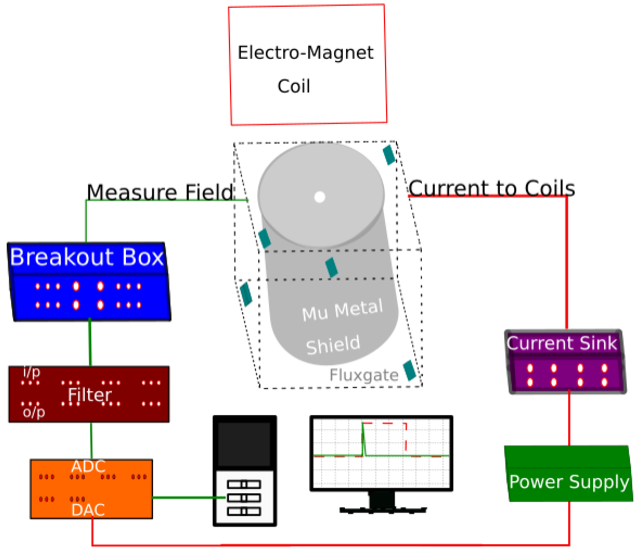
\includegraphics[width=0.4 \textwidth]{Images/exp}
%     \caption[width=0.4 \textwidth]{Schematic diagram of prototype active compensation system at University of Winnipeg . }
%     \label{fig:active shielding}
% \end{figure}
% \begin{figure}
%     \centering
%     \includegraphics[width=0.5 \textwidth]{Images/ss}
%     \caption[width=0.4 \textwidth]{PI loop in flow chart. First measurement from the fluxgates will act as set-point. Then the repeated measurements from the fluxgates are taken. For each measurement difference with the setpoint are noted. On the basis of the difference, the required amount of current for the coils surrounding the outermost layer of the shileding are determined and sent. Those coil currents generate required amount of magnteic flux to compensate for the differences.}
%     \label{fig:active shielding}
% \end{figure}
%  The field fluctuations around the prototype has been found tom $\sim \pm$100 nT. It is also discussed that magnetic fields are normally distributed with standard deviation is 1.5 nT. With this section, Chapter~\ref{ch:amcP} is finished.
